%!TEX root = ../../Master.tex
\section{A* in a Multistory Building Complex}

In this section the A* algorithm will be explained, and the solution to the various problems will be elaborated.

\subsection{Reasoning Behind the use of A*}
The Dijkstra algorithm always finds the shortest route between two positions. But because Dijkstra always calculates every possible path until it gets to the desired destination, a lot of calculations are necessary. If some of these calculations could be avoided, the runtime would be lowered which would suite the usage requirement\cref{irm_tid}. By using A*, the amount of calculations can be reduced because of the logic the algorithm uses, when admissible values are applied correctly.

\subsection{Multiple Layer Handling through FLAWLESS} \label{multlayhan}

When using A* to find a path, the use of a euclidean heuristic becomes problematic when traversing multiple floors in a building. Figure \ref{fig:buildingAstar} helps illustrate this. If a euclidean heuristic is used, the algorithm will, whenever it enters a new floor, move towards the vertex (b) that is directly below the desired goal (a), regardless of whether it is an exit vertex or not. See \cref{e_vertex}. After this point has been reached, the A* algorithm will expand the search from this vertex. This will immensely decrease the usefulness of the euclidean heuristic, to a point where the A* might no longer preferable to Dijkstras algorithm. Because a low runtime is required for the solution, a better way of traversing floors must be employed.

\begin{figure}[ht!]
    \centering
    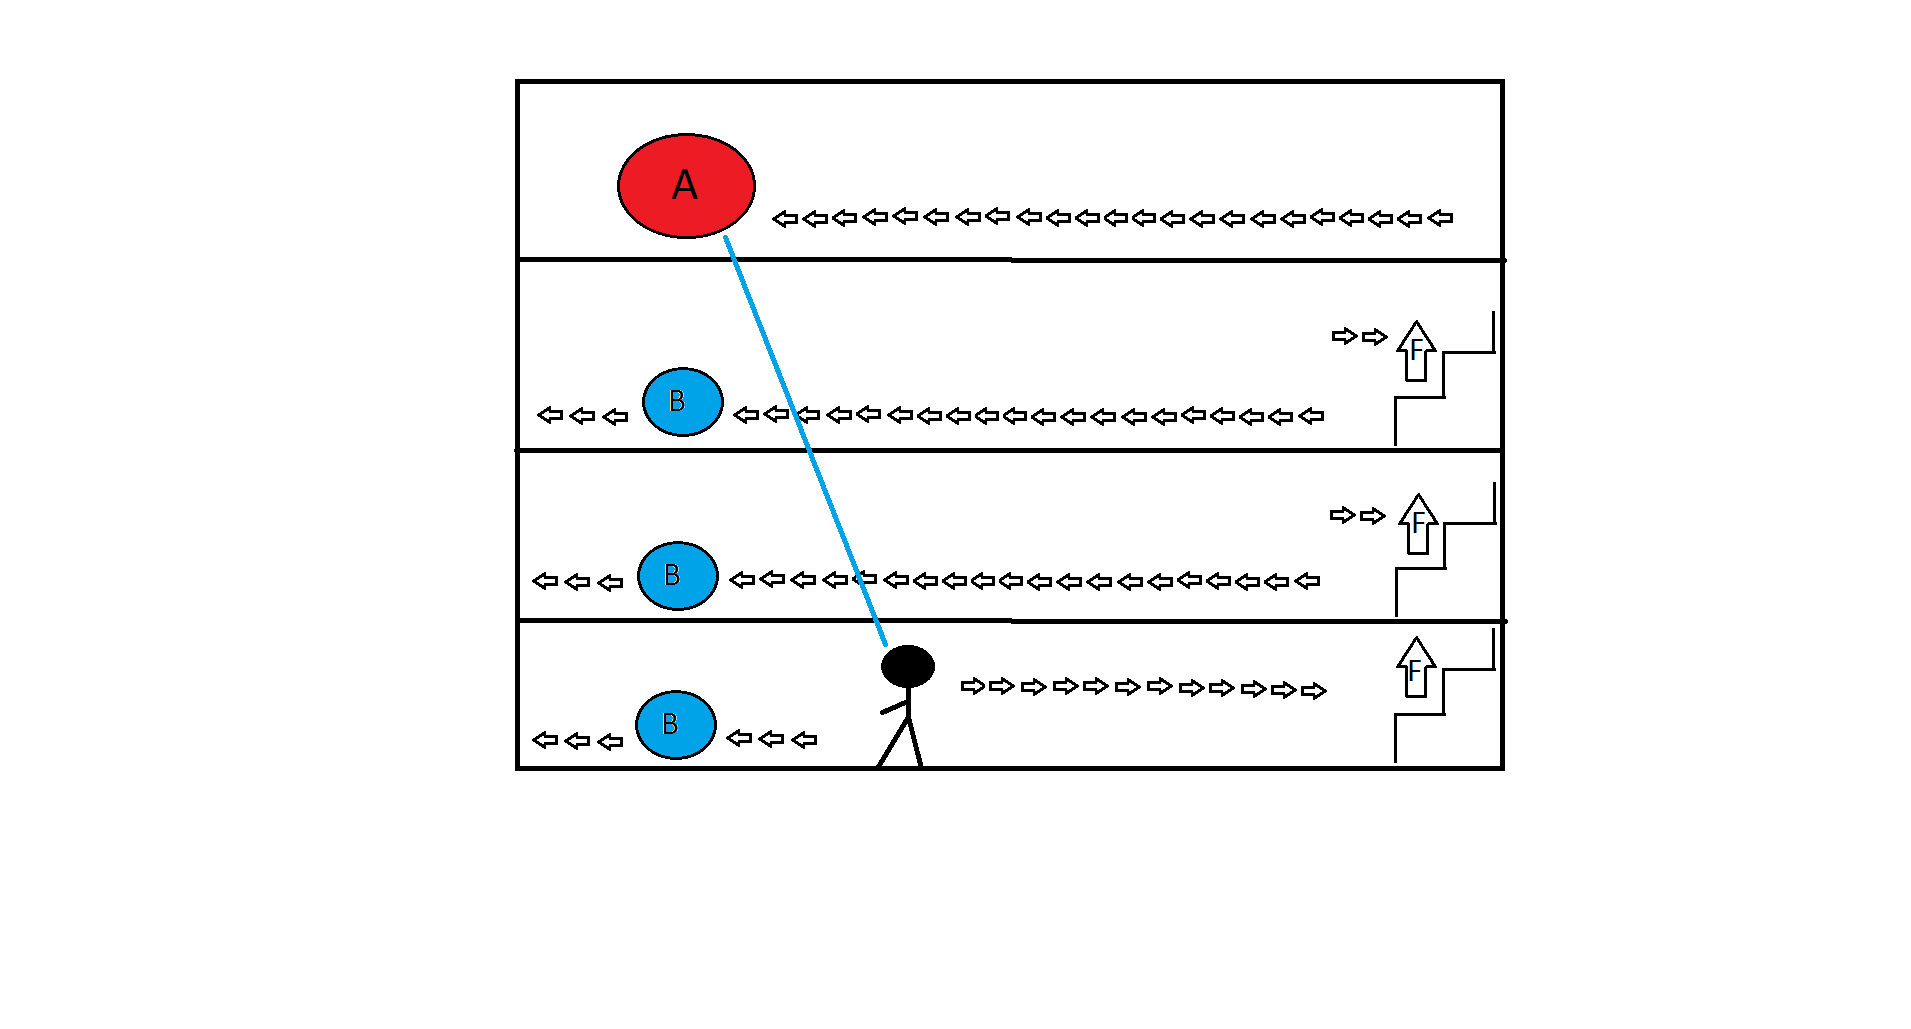
\includegraphics[width=0.5\textwidth]{buildingastar_paint}
    \caption{How many vertices the A* algorithm would expand, if using the euclidean distance as heuristic}
    \label{fig:buildingAstar}
  \end{figure}

The solution to this problem lies in a tripartitioning of the pathfinding process, and is illustrated in \cref{fig:flawless1,fig:flawless2,fig:flawless3}. Using the fact that the optimal route from one exit vertex to any other exit vertex is static, and only the choice of exit vertices varies when finding the optimal route between the intial and final floor, the paths from exit vertex to exit vertex can be precomputed. By computing and storing these routes when initializing the program, the response time when prompted for a path, will be lowered significantly.

When using this approch, the precalculation is executed at system startup using Dijkstras algorithm, in order to get the optimal connections between all exit vertices. There is no need for a faster algorithm, since there is no user communication during this calculation.

\begin{figure}[ht!]
    \centering
    \includegraphics[width=0.5\textwidth]{flawless1}
    \caption{Illustration of the precomputation of routes between the floors}
    \label{fig:flawless1}
  \end{figure}

The runtime will consist of a round of A* runs done on both the intial floor and the destination floor. These runs are done from the start vertex and the destination vertex to all exit vertices on their respective floors. 

\begin{figure}[ht!]
    \centering
    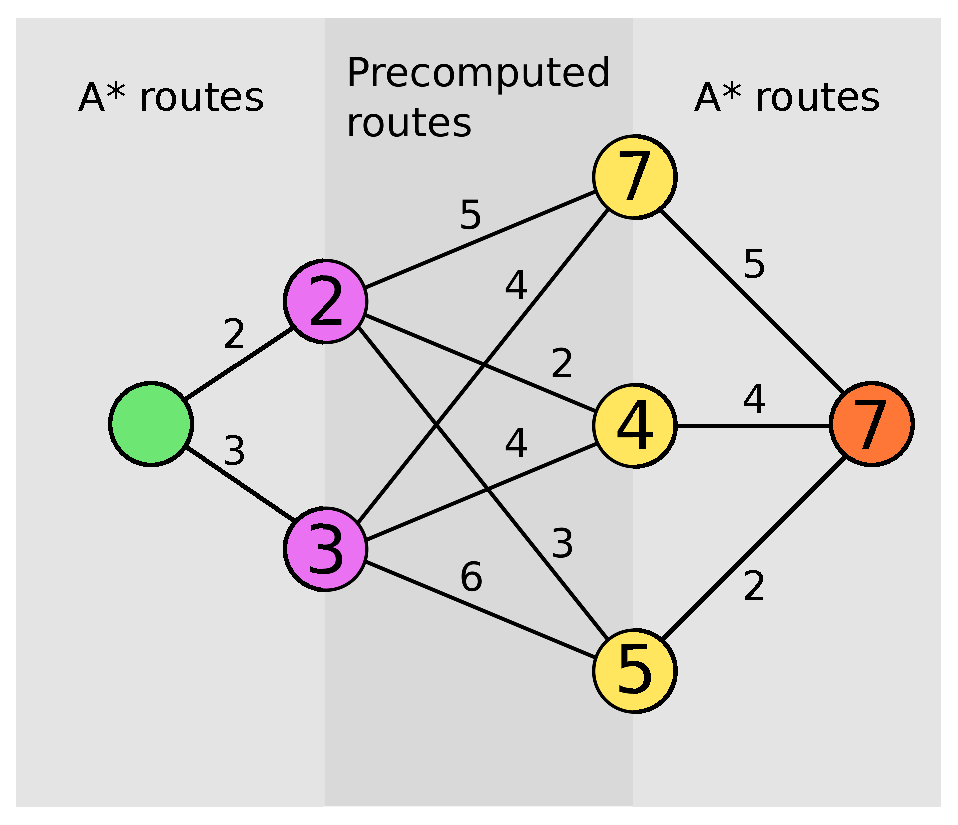
\includegraphics[width=0.5\textwidth]{flawless3}
    \caption{Illustration of the A* runs}
    \label{fig:flawless2}
  \end{figure}

When this has been computed, all the possible combinations of paths will have their individual evaluation values added, and a comparison between the total evaluation values will dertermine the optimal path across the multiple floors. 

\begin{figure}[ht!]
    \centering
    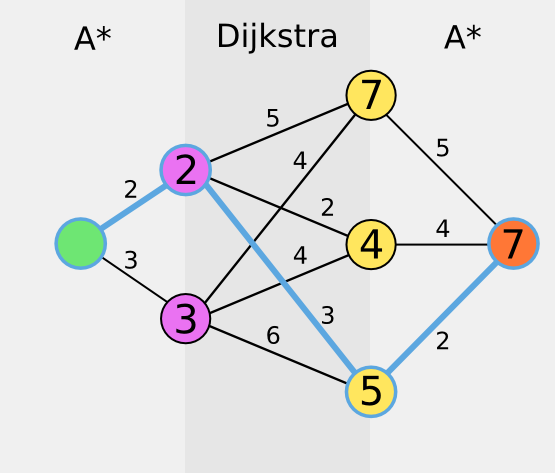
\includegraphics[width=0.5\textwidth]{flawless4}
    \caption{Illustration of the added evaluation values, and the route that is chosen}
    \label{fig:flawless3}
  \end{figure}

This method of handing multiple floors in a building is named fused locale A* with level-calculation executed at system startup, and shortened to FLAWLESS.


\subsection{Choosing Stairs or the Elevator}

When the algorithm decides whether to choose stairs over elevators when traveling to another floor, the choice is determined by the weight of the route. The weight is based on how time consuming or psychical fatiguing the process is for the user. In order to weight the vertex in a way that reflects reality the stairs weight should grow exponentially. The more stairs a user climbs in succession the more psychical fatiguing it gets which is the reasoning for the exponential growth. This has however been delimited in \cref{sec:delimination} and both the stairs and elevator will therefore be weighted in a linear manner. \Cref{fig:labeled_stairsVSelevators} shows a graph with the stairs and elevator. The elevator starts with a higher initial weight as it takes time to enter the elevator and select a destination floor. In contrast the stairs start ascending as soon the user is on the first step. But once the user is inside the elevator, and it starts ascending, it will catch up on the stairs and eventually become the fastest way of travelling. On the graph, the point where the elevator is faster than the stairs, is where the two lines cross, which in this case is between the fourth and third floor. This means if the user has to travel four or more floors, the planned route should utilize the elevator.

\begin{figure}[ht!]
    \centering
    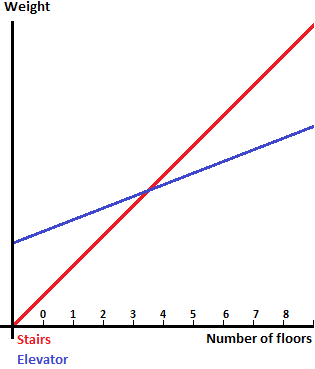
\includegraphics[width=0.5\textwidth]{stairsVSelevators.png}
    \caption{}\label{fig:labeled_stairsVSelevators}
  \end{figure}


In \cref{sec:interusers} different people have been described each with their own characteristics, and as concluded, some people don't have the opportunity to take the elevators or the stairs. 

To avoid adding a specific vertex such as an elevator or a stair, the weight connecting this specific vertex is mulitplied with an extremely high number. This means that when the search algorithm travels through the graph, it will not consider e.g. the stairs.
Another way of resolving the problem is to stop the algorithm from considering the specified vertex is by disabling it. That way the algorithm will never visit this vertex. A problem with this is if the disabled vertex is the only way to the destination.



